\chapter{Atomic and Molecular Mass}

%fixme add hook

Let's look at the different information shown on a periodic tile:

\begin{center}
\includegraphics[width = 4in]{element.png}
%fixme change "weight" to "mass" or remake image
\end{center}

The four things we learn from a periodic tile are:
\begin{enumerate}
\item the symbol: as discussed in the previous chapter, each element has a unique symbol. Element symbols are used when showing the structure of a molecule and modeling chemical reactions. 
\item the atomic number: this is also unique for each element. Take a look at the periodic table a few pages forward. Every tile has a unique atomic number, and the tiles are laid out in a generally increasing atomic number (you'll learn why the periodic table is arranged this way in Sequence 2). 
\item the atomic mass: this is the average mass of all the atoms of that element in existence. Just like your overall grade in a class is the weighted average of all the individual grades you earned, atomic mass is the weighted average of the masses of all the individual atoms of that element. 
\item the name: not all periodic tables show the name of an element on its tile. This is why it is useful to know the symbols of common elements. 
\end{enumerate}

Recall from the previous chapter that we classify atoms by the number of protons they have. What this means is that if we want to know what element an atom is, we have to look at the number of protons. Take a look at the three carbon atoms below and note what is the same and what is different among them:

\begin{center}
\includegraphics[scale=0.35]{carbon_iso.png}
\end{center}

These different versions of carbon all have 6 protons, which is also carbon's atomic number. This isn't a coincidence: the atomic number \textit{is} the number of protons in every atom of an element. If I tell you an atom has 4 protons, you would find atomic number 4 and see that the element is beryllium. To know how many protons an oxygen atom has, you would find its tile and see that it has atomic number 8. 

Ok, so now we know atoms of the same element have the same number of protons, and that number is given by the element's atomic number. The difference between these carbon atoms explains the other number on a periodic tile: the atomic mass. 



A proton and a neutron have about the same mass. An electron, on the
other hand, has much less mass: One neutron weighs about the same
amount as 2000 electrons. This means that the mass of any object comes mostly
from the protons and neutrons in the nucleus of its atoms. \index{proton} \index{neutron}

We know how many protons an atom has by what element it is, but how do we know the 
number of neutrons?

If you fill a balloon with helium, it will have two different
kinds of helium atoms. Most of the helium atoms will have 2 neutrons, but a
few will have only 1 neutron. We say that these are two different
\textit{isotopes} of helium. We call them helium-4 (or $^4He$) and
helium-3 (or $^3He$). Isotopes are named for the sum of protons and
neutrons the atom has: helium-3 has 2 protons and 1 neutron.\index{isotopes}

A hydrogen atom nearly always has just 1 proton and no neutrons. A
helium atom nearly always has 2 protons and 2 neutrons. So, if you
have a 100 hydrogen atoms and 100 helium atoms, the helium will have
about 4 times more mass than the hydrogen. We say ``Hydrogen is about
1 atomic mass unit (amu), and helium-4 is about 4 atomic mass
units.''\index{atomic mass unit}

What, precisely, is an atomic mass unit? It is defined as 1/12 of
the mass of a carbon-12 atom. Scientists have measured the mass of
helium-4, and it is about 4.0026 atomic mass units. (By the way, an
atomic mass unit is also called a \textit{dalton}.)

\pagebreak

%final above, pieces below
Now you are ready to take a good look at the periodic table of
elements. Here is the version from Wikipedia:\index{periodic table of elements}

\includegraphics[width=0.75\textwidth]{periodic.png}

% ADD: Periodic Trends, Periods, Collums, Atomic Radius, Electronegativity,

\pagebreak
There is a square for each element. In the middle, you can see the atomic
symbol and the name of the element. In the upper-right corner is the
atomic number --- the number of protons in the atom.

In the upper-left corner is the atomic mass in atomic mass units.\index{atomic mass}

\includegraphics[width=0.8\textwidth]{element.png}

Look at the atomic mass of boron. About 80\% of all boron atoms have
six neutrons. The other 20\% have only 5 neutrons. This difference is why most boron atoms
have a mass of about 11 atomic mass units, but some have a mass of
about 10 atomic mass units. The atomic mass of boron is equivalent to the average
mass of a boron atom: 10.811.
% ADD: Talk about mass spectroscopy
%\includegraphics[width=0.75\textwidth]{KA_Mass_Spectroscopy_Zr.png}

\begin{Exercise}[title={Mass of a Water Molecule}, label=water_mass]

Using the periodic table, what is the average mass of one water molecule in atomic mass units?

\end{Exercise}
\begin{Answer}[ref=water_mass]

  The average hydrogen atom has a mass of 1.00794 atomic mass units.

  The average oxygen atom has a mass of 15.9994.

  $2 \times 1.00794 + 15.9994 = 18.01528$ atomic mass units.

\end{Answer}

\section{xfer from intro chapter} 
fixme integrate into this chapter
\subsection{Reading the Periodic Table}
The Periodic Table organizes what we know about the structure of different
elements. Each element has its own block or tile on the Periodic Table, and the
information on the tile tells us about the structure of that atom. Take a look at
the tile for carbon:

\begin{center}
%\includegraphics[width=2in]{carbon_tile.png}
\end{center}

The letter (or letters, as is the case for other elements) is the atomic symbol
for the element. There are two key numbers: the atomic number and the average
atomic mass. For carbon, the atomic number is 6 and the average atomic mass is
12.011. The atomic number tells us how many protons there are in the nucleus of
any atom of carbon. Since every element has a unique number of protons, every
element has a unique atomic number. All carbon atoms have 6 protons. The other
number is the average atomic mass - it tells us the weighted average of the
mass of all the carbons in the universe. When the average atomic mass is in
a whole number, as it is for polonium, it means that the element is very unstable.
As a result, the mass given is the mass of the most stable isotope (we'll talk
more about stability and isotopes below). On some periodic tables, the mass
number of the most stable isotope will be in parentheses or brackets. In
summary, if the larger number is a whole number, it is the mass number; if it
is a decimal (even if the decimal ends in .00), it is the average atomic mass,
which we will discuss further below.

\begin{center}
%\includegraphics[width=2in]{polonium_tile.png}
\end{center}

The Royal Society of Chemistry has a very useful interactive periodic table:
periodic-table.rsc.org. We can use the periodic tile for an element to
determine the number of protons, electrons, and most common number of neutrons
for a neutral atom of that element (we'll explain why the periodic tile tells
us the "most common number of neutrons" below).

\textbf{Example}: State the atomic symbol for and the number of protons,
neutrons, and electrons in a neutral atom of plutonium.

\textbf{Solution}: The plutonium tile on your periodic table should look
something like this:
\begin{center}
   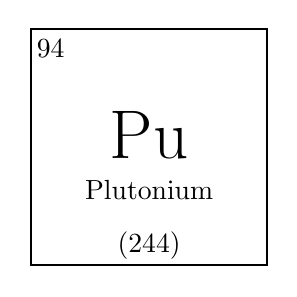
\begin{tikzpicture}
        \draw[black, thick] (-1.5, -1.5) rectangle (1.5,1.5);
        \node[font = \Huge] at (0,0.15) {Pu};
        \node[] at (-1.25, 1.25) {$94$};
        \node[] at (0, -0.55) {Plutonium};
        \node[] at (0, -1.25) {$(244)$};
    \end{tikzpicture}
\end{center}

[The information may be arranged differently, but you should at least see the
symbol and two numbers.] As you can see, the atomic symbol for plutonium is Pu.
Since its atomic number is 94, we know every atom of plutonium has 94 protons.
To know the number of electrons, we will take advantage of the fact that the
question is asking about a \textit{neutral} atom. This means there are the same
number of positive charges as negative charges. So, since there are 94 protons,
a neutral atom of plutonium must have 94 electrons (each proton has a +1 charge
and each electron has a -1 charge). Lastly, let's determine the number of
neutrons. The other number, 244, is the mass number. It represents the total
number of protons and neutrons in the nucleus. Since we know plutonium has 94
protons, we can find the number of neutrons by subtracting the atomic number
from the mass number:

\begin{center}
   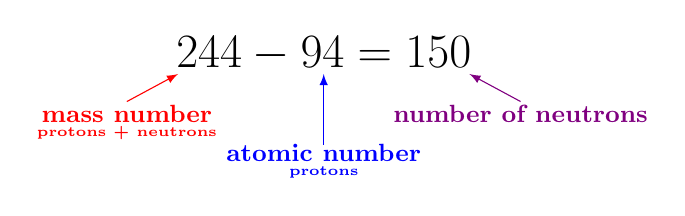
\begin{tikzpicture}
        \node[font = \LARGE] at (0,0) {$244 - 94 = 150$};
        \node[font = \small, red] at (-2.5, -0.75) {\textbf{mass number}};
        \node[font = \tiny, red] at (-2.5, -1) {\textbf{protons + neutrons}};
        \draw[red, -latex] (-2.5, -0.6) -- (-1.85, -0.25);
        \node[font = \small, blue] at (0, -1.25) {\textbf{atomic number}};
        \node[font = \tiny, blue] at (0, -1.5) {\textbf{protons}};
        \draw[blue, -latex] (0, -1.15) -- (0, -0.25);
        \node[font = \small, violet] at (2.5, -0.75) {\textbf{number of neutrons}};
        \draw[violet, -latex] (2.5, -0.6) -- (1.85, -0.25);
    \end{tikzpicture}
\end{center}

Therefore, an atom of plutonium has 150 neutrons. Now let's address how to find
the number of neutrons when the periodic tile shows an average atomic mass,
instead of a mass number. This occurs when there is more than one "version" of
an element. In the case of plutonium, there is only one version, which is why
the periodic tile shows a mass number instead of an average atomic mass. To
learn about average atomic mass, we will use carbon as an example.

Have you heard of carbon-14 dating? The phrase "carbon-14" refers to a rare
type of carbon that decays radioactively. By seeing how much carbon-14 has
decayed, scientists can estimate the age of organic materials, such as bone or
ash. Carbon-14 is a radioactive isotope (or version) of carbon. The 14 refers to
the mass number - the total amount of protons and neutrons in the nucleus
(sometimes, we shorten the isotope name by just using the atomic symbol, in
this case C-14). Isotopes are versions of an element with different numbers of
neutrons. The atomic number is the same for them all - they all have the same
number of protons. But the different number of neutrons causes different
isotopes to have different masses. Examine the models of carbon-12, carbon-13,
and carbon-14 below. What is different between them? What is the same?



You should have noticed that all three atoms have 6 protons and 6 electrons,
while they have differing numbers of neutrons. The most common isotope of carbon
is carbon-12, with 6 protons and 6 neutrons in its nucleus. Carbon-14, on the
other hand, has 8 neutrons, which makes the nucleus unstable, leading to
radioactive decay. The average atomic mass
is the weighted average of all the carbon atoms in existence. Since the vast
majority of carbon is carbon-12, the average atomic mass is very close to 12.
You cannot determine the mass number of an individual atom from the periodic
table; it only tells you the average of all the isotopes. However, especially
for light atoms (atoms in the first two rows of the periodic table), you can
usually determine the mass number of the most common isotope by rounding the
average atomic mass to the nearest whole number.

\textbf{Example}: Germanium has atomic symbol Ge. State the number of protons,
number of electrons, and most common number of neutrons in a neutral atom of
germanium.

\textbf{Solution}: Examining the periodic table, we see that germanium has an
atomic number of 32, which means a neutral atom of germanium has 32 protons and
32 electrons. The average atomic mass is 72.630, which rounds up to 73. So, the
most common isotope of germanium is Ge-73, which has $73 - 32 = 41$ neutrons.

\begin{Exercise}[title = {Determining Numbers of Subatomic Particles}, label = pne]
Use a periodic table to complete the table below (assume neutral atoms): %fixme wrap text for neutrons column

\begin{tabular}{|c|c|c|c|c|}
\hline\\
Element Name & Atomic Symbol & Protons & Most Common Number of Neutrons & Electrons\\\hline
 & Fr & & & \\\hline
 & & & & 33\\\hline
 Erbium & & & & \\\hline
  & & 48 & & \\\hline
\end{tabular}
\end{Exercise}

\begin{Answer}[ref = pne]
\begin{tabular}{|c|c|c|c|c|}
\hline\\
Element Name & Atomic Symbol & Protons & Most Common Number of Neutrons & Electrons\\\hline
 Francium & Fr & 87 & 136 & 87 \\\hline
 Arsenic & As & 33 & 42 & 33 \\\hline
 Erbium & Er & 68 & 99 & 68 \\\hline
 Cadmium & Cd & 48 & 64 & 48 \\\hline
\end{tabular}
\end{Answer}

\section{Molar Mass}

An atomic mass unit is a very, very, very small unit; we would much
rather work in grams. It turns out that $6.02214076 \times 10^{23}$
atoms equal 1 mole (a standard measure for chemistry). Scientists use this number so often
that they gave it a name: \textit{the Avogadro constant} or
\textit{Avogadro's number}.\index{Avogadro's number}



If you have 12 doughnuts, that's a dozen doughnuts. If you have
$6.02214076 \times 10^{23}$ doughnuts, you have a \textit{mole} of
doughnuts. This isn't really a practical measurement, as a mole of doughnuts would be about the size of the earth. We use
moles for small things like molecules.\index{mole}


Let's say you want to know how much a mole of $NaCl$ weighs. From the
periodic table, you see that $Na$ has an atomic mass of 22.98976
atomic mass units, and $Cl$ has 35.453 atomic mass units.  One atom of
$NaCl$ has a mass of $22.98976 + 35.453 = 58.44276$ atomic mass units.
This means a mole of $NaCl$ has a mass of $58.44276$ grams. Handy, right?
% ADD: Conversions should probably come before this

\begin{Exercise}[title={Burning Methane}, label=burning_methane]

Natural gas is mostly methane ($CH_4$). When one molecule of methane
burns, two oxygen molecules ($O_2$) are consumed. One molecule of
$H_2O$ and one molecule of $CO_2$ are produced.
% ADD: Need to explain mole to mole ratios first, Law of Divine Proportion
% ADD: Include Significant Figures

If you need 200 grams of water, how many grams of methane do you need
to burn?

(This is how the hero in ``The Martian'' made water for his garden.)


\end{Exercise}
\begin{Answer}[ref=burning_methane]

From the last exercise, you know that 1 mole of water weighs 18.01528
grams, meaning 200 grams of water is about 11.1 moles. So you need to burn
11.1 moles of methane.

What does one mole of methane weigh? Using the periodic table:
$12.0107 + 4 \times 1.00794 = 16.04246$ grams.

$16.0424 \times 11.10 = 178.1$ grams of methane.

\end{Answer}

\section{Heavy atoms aren't stable}

When you look at the periodic table, there are a surprisingly large
number of elements. You might be told to ``Drink milk so that you can
get the calcium you need.'' However, no one has told you ``You should
eat kale so that you get enough copernicium in your diet.''

Copernicium, with 112 protons and 173 neutrons, has only been observed
 in a lab. It is highly radioactive and unstable (meaning it decays). A copernicium
atom usually lives for less than a minute before decaying.
% ADD: Half Life

The largest stable element is lead, which has 82 protons and between
122 and 126 neutrons. Elements with lower atomic numbers than lead,
have at least one stable isotope, while elements with higher atomic numbers
than lead don't.

Bismuth, with an atomic number of 83, is \textit{almost} stable. In fact, most
bismuth atoms will live for billions of years before decaying!
